\section{Experimentación}

Dada una cantidad de vértices, los grafos se generan con formato DIMACS \footnote{Para ver algunos ejemplos del formato: http://mat.gsia.cmu.edu/COLOR/instances.html}. El generador toma como parámetro la densidad del grafo. Dada una clique con esa cantidad de vértices, se elijen vértices al azar hasta que se llega a la densidad deseada. Debido a que estas instancias están diseñadas para coloreo de grafos, asignamos los vértices de forma uniforme en el total de particiones pasado por parámetro a nuestro programa de coloreo particionado.

Por cuestiones de tiempo, para cada una de las experimentaciones CPLEX se ejecuto sin limtar la cantidad de threads con un procesador Intel(R) Core(TM) i7-3610QM CPU @ 2.30GHz y 16GB de memoria RAM.

\subsection{Eliminación de simetría}

Al igual que el problema de coloreo de grafos, el problema del coloreo particionado de grafos presenta una gran cantidad de soluciones simétricas. De no romper la simetría del problema, los algoritmos de búsqueda normalmente tendrían un espacio mucho mayor de búsqueda, lo que afecta el tiempo de ejecución de forma considerable a medida que crece el tamaño del problema. Para romper la simetría en nuestro problema, en la sección \ref{simetria} mostramos como utilizamos la clásica condicion de coloreo de que los colores se deben utilizar en orden. Esto se puede ver en el siguiente gráfico:

\begin{figure}[h]
\centering
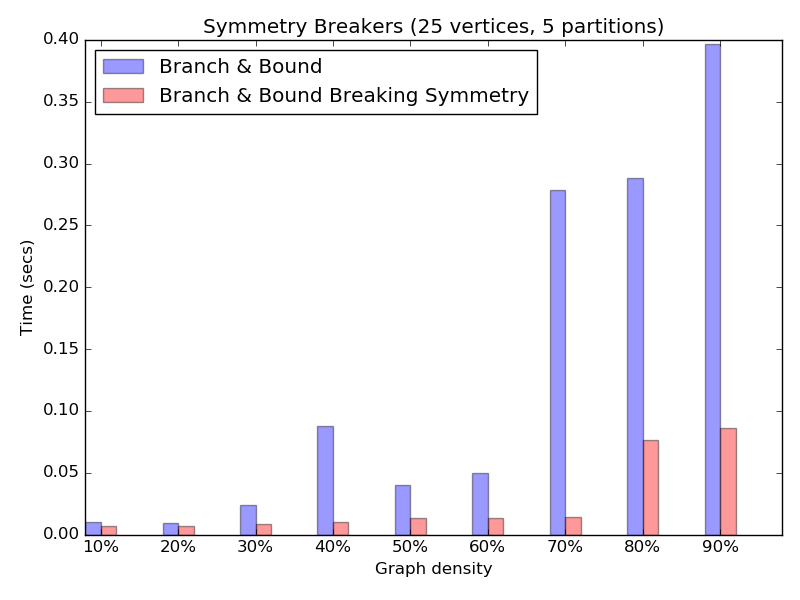
\includegraphics[scale=0.7]{img/2-symmetry_v25_p5_l40_t1_b0.png}
\caption{Eliminación de simetría.}
\end{figure}

Esto nos da una noción sumamente relevante de la importancia y la efectividad de romper la simetría en los LP. Cabe mencionar que existen muchas otras estrategias para romper la simetría de los problemas, y esta no es necesariamente la mejor.

\pagebreak

\subsection{Efectividad de las familias de desigualdades}

La idea de este experimento fue comparar las diferentes estrategias de planos de corte. Para ello se tomo a 40 como el a la cantidad de cortes de cada tipo que se podían agregar, con una sola iteración:

\begin{figure}[h]
  \centering
  \begin{minipage}[b]{0.49\textwidth}
    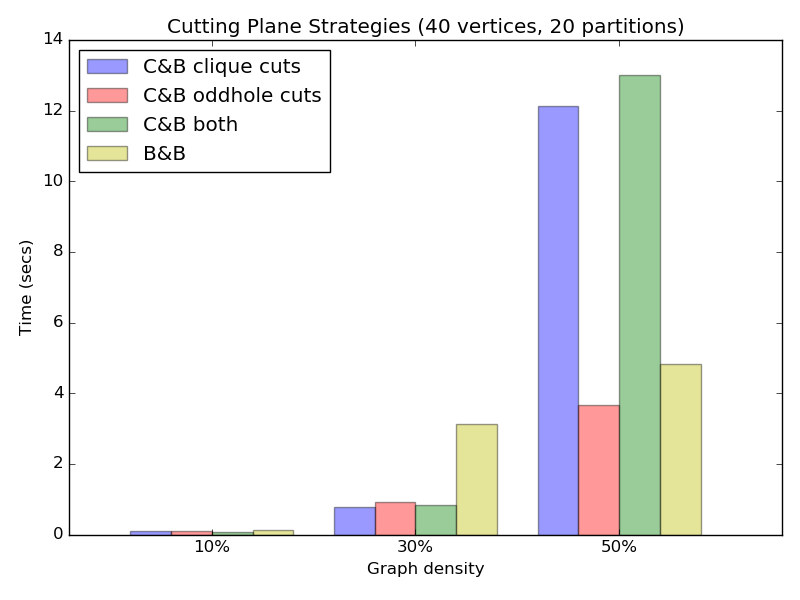
\includegraphics[width=\textwidth]{img/5-cuts_v40_p20_i1_l40_t1_b0.png}
    \caption{Estrategias de planos de corte (tiempo)}
  \end{minipage}
  \hfill
  \begin{minipage}[b]{0.49\textwidth}
    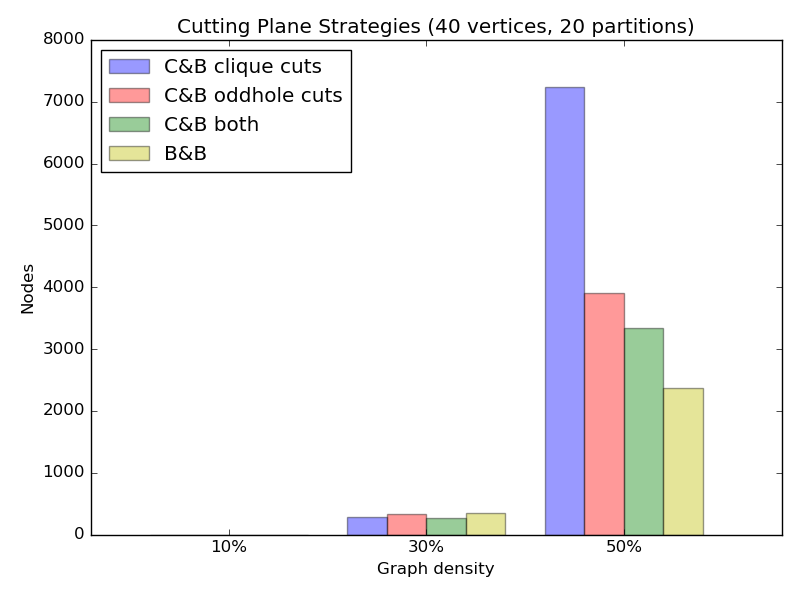
\includegraphics[width=\textwidth]{img/5-cuts_v40_p20_i1_l40_t1_b0_nodes.png}
    \caption{Estrategias de planos de corte (nodos recorridos)}
  \end{minipage}
\end{figure}

Lo primero que podemos observar que no siempre hay una estrategia ganadora. Claramente la estrategia a seguir depende de la densidad del grafo. Cuanto mas denso, mas cliques nuestra heurística podría encontrar y a priori uno esperaría que los tiempos mejoren. Esto no sucede, y de hecho agregar las restriciones de clique empeora el tiempo de ejecución con respecto al resultado de B\&B. También podemos observar que mejor tiempo de ejecución no necesariamente implica que se recorren menos nodos del árbol de enumeración. En contra de lo que esperábamos, las desigualdades de agujero impar parecen funcionar bien, aunque por supuesto se debe llevar a cabo una experimentación mas exhaustiva.

\subsection{Efecto de aumentar el numero de particiones}

A medida que aumentamos el numero de particiones, el problema comienza a ser mas difícil y a parecerse mas a uno de coloreo. Esto lo podemos ver en el siguiente gráfico. Para Cut \& Branch, solo utilizamos los mejores 40 cortes de clique con una iteración. A medida que el problema se hace mas difícil, podemos observar como la ganancia del corte es mayor.

\begin{figure}[h]
  \centering
  \begin{minipage}[b]{0.49\textwidth}
    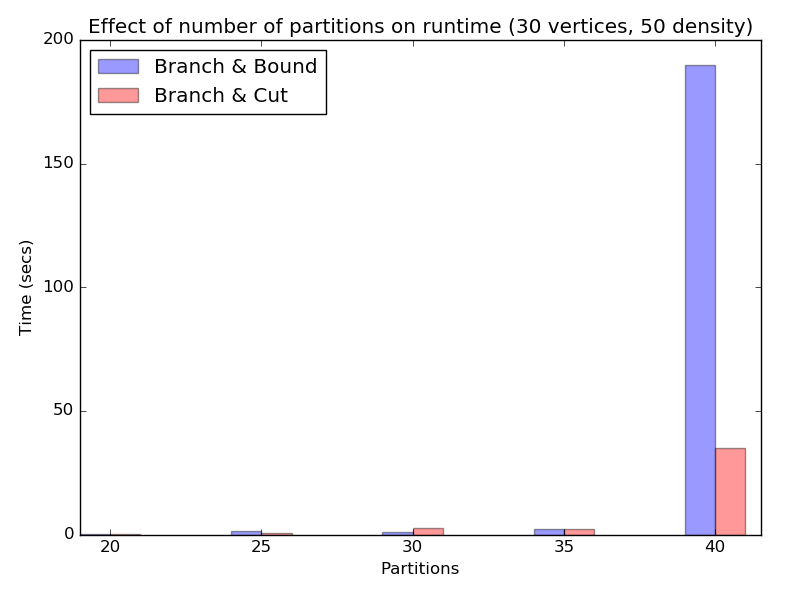
\includegraphics[width=\textwidth]{img/3-partitions_v30_d50_i1_co0_l40_t1_b0.png}
    \caption{Tiempo de ejecucion a medida que aumenta el numero de particiones.}
  \end{minipage}
  \hfill
  \begin{minipage}[b]{0.49\textwidth}
    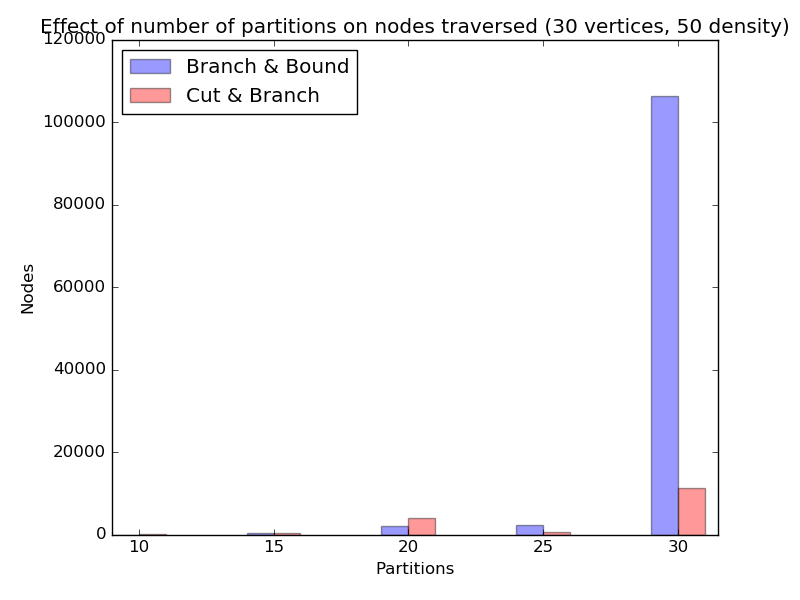
\includegraphics[width=\textwidth]{img/3-partitions_v30_d50_i1_co0_l40_t1_b0_nodes.png}
    \caption{Nodos recorridos a medida que aumenta el numero de particiones.}
  \end{minipage}
\end{figure}

\pagebreak

\subsection{Efecto de aumentar la densidad del grafo}

\begin{figure}[h]
  \centering
  \begin{minipage}[b]{0.49\textwidth}
    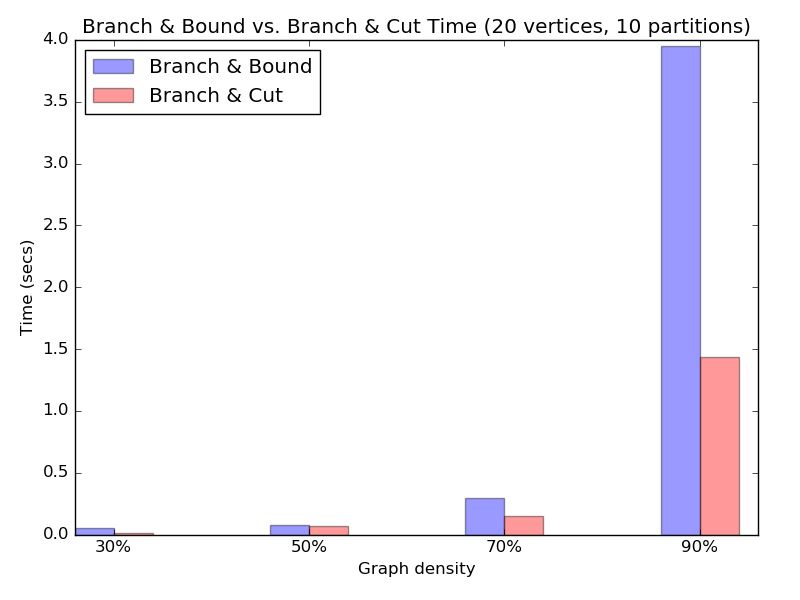
\includegraphics[width=\textwidth]{img/1-bb_vs_bc_v20_p10_i1_co0_l40_t1_b0.png}
  \end{minipage}
  \hfill
  \begin{minipage}[b]{0.49\textwidth}
    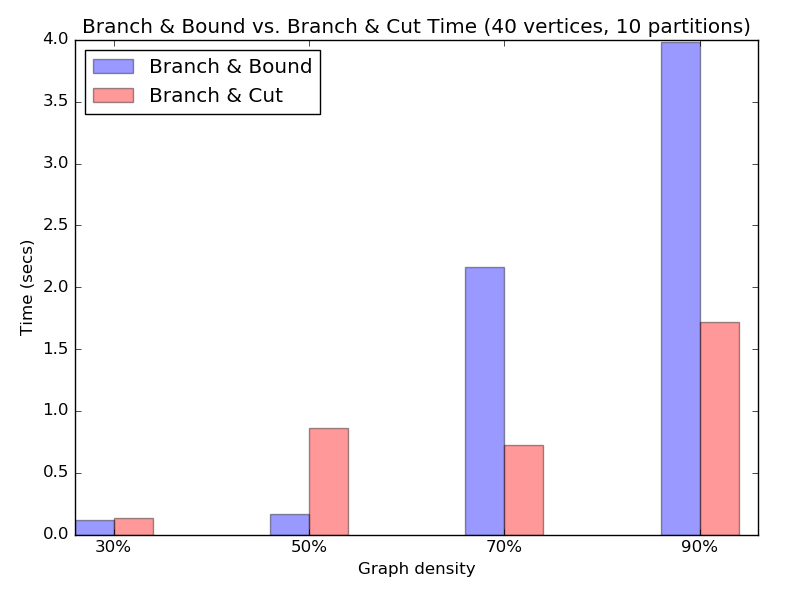
\includegraphics[width=\textwidth]{img/1-bb_vs_bc_v40_p10_i1_co0_l40_t1_b0.png}
  \end{minipage}
  \begin{minipage}[b]{0.49\textwidth}
    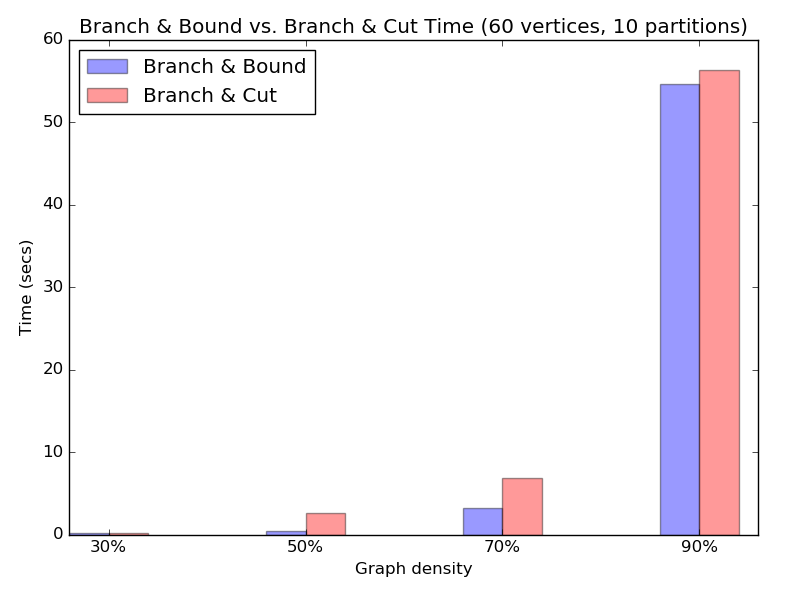
\includegraphics[width=\textwidth]{img/1-bb_vs_bc_v60_p10_i1_co0_l40_t1_b0.png}
  \end{minipage}
  \hfill
  \begin{minipage}[b]{0.49\textwidth}
    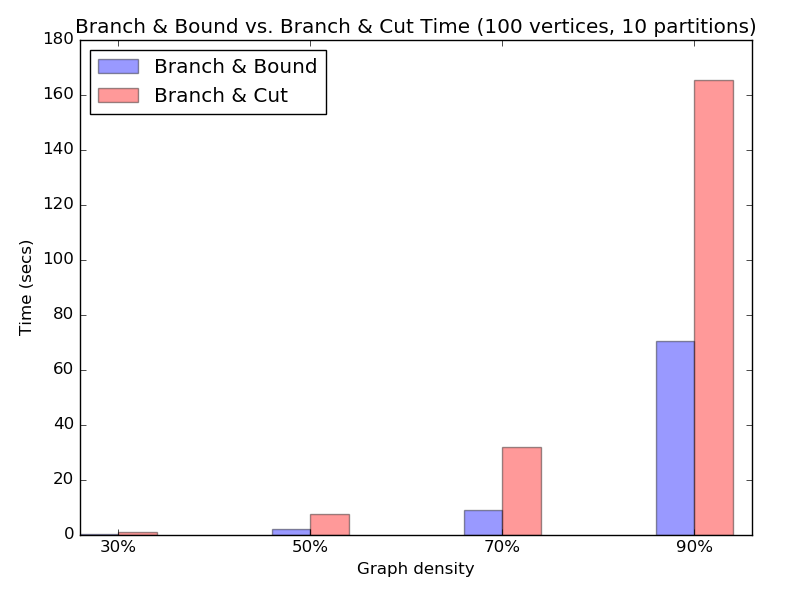
\includegraphics[width=\textwidth]{img/1-bb_vs_bc_v100_p10_i1_co0_l40_t1_b0.png}
  \end{minipage}
	\caption{Efecto de aumentar la densidad del grafo.}
\end{figure}

A medida que aumenta la densidad del grafo, la dificultad del problema es claramente mayor. En los casos donde el numero de particiones es mayor en relación al numero de vértices, Branch \& Cut con 1 iteración y 40 desigualdades violadas parece funcionar mejor. Esto no sucede en grafos esparsos, donde Branch \& Bound puro tiene un menor tiempo de ejecución.

\pagebreak

\subsection{Efecto de aumentar la cantidad de restricciones incorporadas por iteración}

Para todos nuestros experimentos en general utilizamos solo 1 iteración con un limite de 40 desigualdades por familia. La idea de este experimento fue evaluar esta configuración. Para ello utilizamos un grafo con 40 vértices y 20 particiones.

\begin{figure}[h]
  \centering
  \begin{minipage}[b]{0.49\textwidth}
    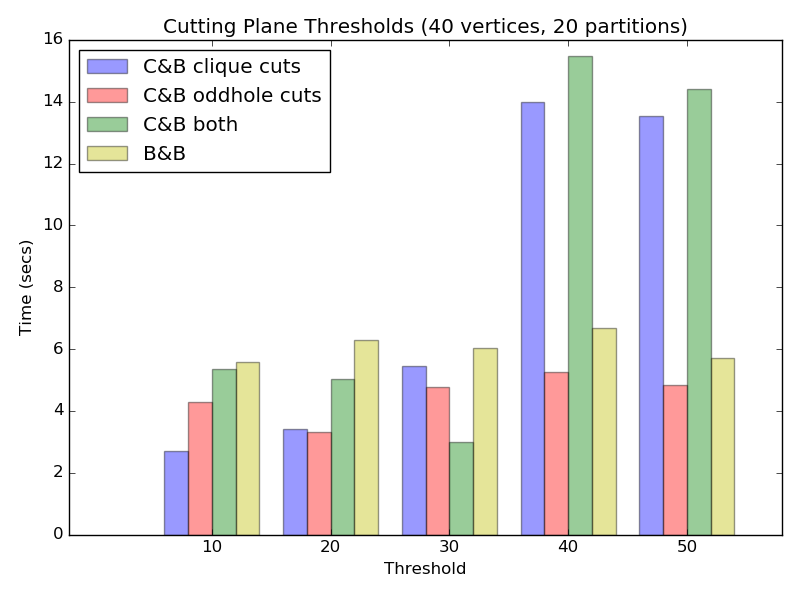
\includegraphics[width=\textwidth]{img/6-thresholds_v40_p20_i1_t1_b0.png}
    \caption{Tiempo de ejecución al incrementar el numero de restricciones incorporadas.}
  \end{minipage}
  \hfill
  \begin{minipage}[b]{0.49\textwidth}
    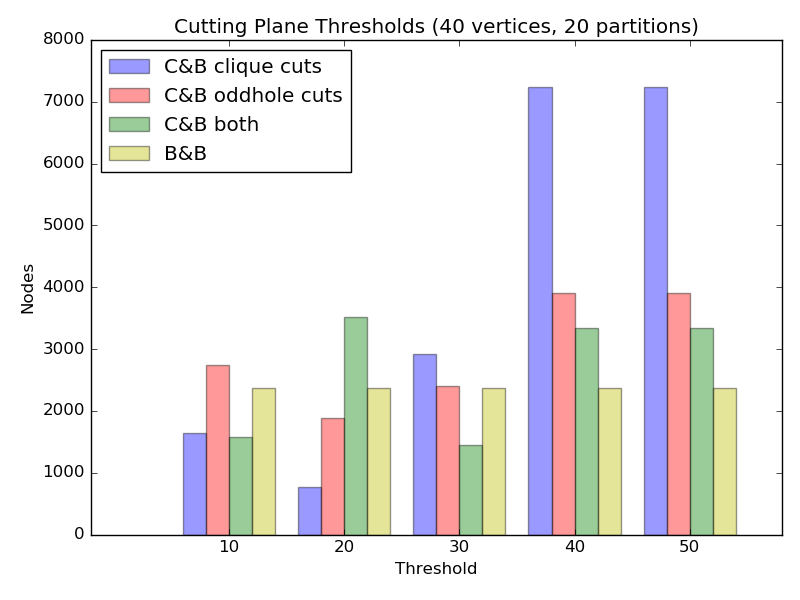
\includegraphics[width=\textwidth]{img/6-thresholds_v40_p20_i1_co2_t1_b0_nodes.png}
    \caption{Nodos recorridos al incrementar el numero de restricciones incorporadas.}
  \end{minipage}
\end{figure}

Como podemos observar, agregar mas restricciones no es siempre ventajoso. En un principio, agregar restricciones parece mejorar la ejecución del C\&B, pero ya a partir de 40 el tiempo de ejecución empeora de forma abrupta para las cliques. Esto no sucede para las restricciones de agujero impar. Nuevamente, esto se puede deber a que nuestra heurística de clique no es lo suficientemente buena.

\subsection{Efecto de aumentar la cantidad de iteraciones de planos de corte}

\begin{figure}[h]
\centering
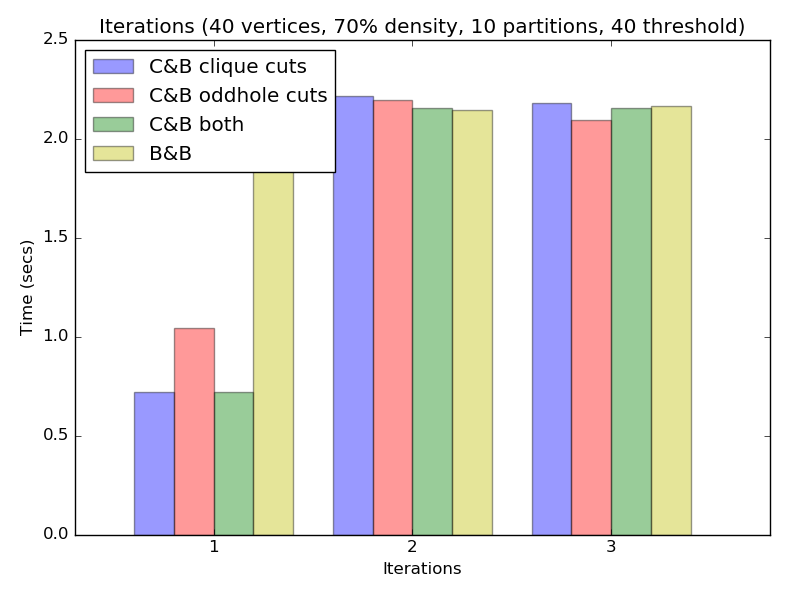
\includegraphics[scale=0.5]{img/7-iterations_v40_p10_l40_t1_b0.png}
\caption{Tiempo de ejecución al aumentar la cantidad de iteraciones de planos de corte.}
\end{figure}

Como podemos ver, aumentar el numero de iteraciones de planos de corte no necesariamente mejora el tiempo de ejecución. En cada iteración lo que hacíamos era generar una familia en función de la solución de la relajación del problema, y luego agregar las \textit{mejores} restricciones. En relación a la sección anterior, esto también esta relacionado con el $threshold$ que elegimos para hacer la experimentación.

\pagebreak

\subsection{Comparación B\&B, C\&B, CPLEX default}

\begin{figure}[h]
  \centering
  \begin{minipage}[b]{0.49\textwidth}
    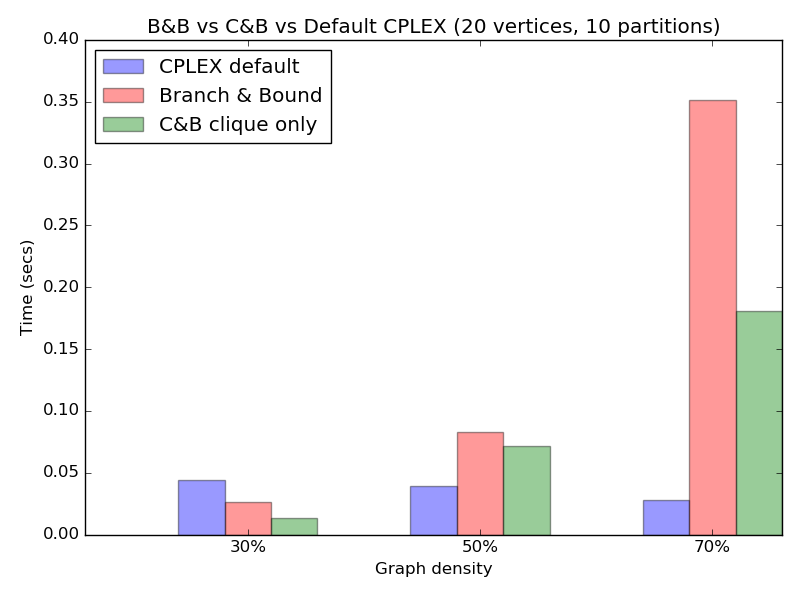
\includegraphics[width=\textwidth]{img/8-compare_v20_p10_i1_l40_t1_b0.png}
  \end{minipage}
  \hfill
  \begin{minipage}[b]{0.49\textwidth}
    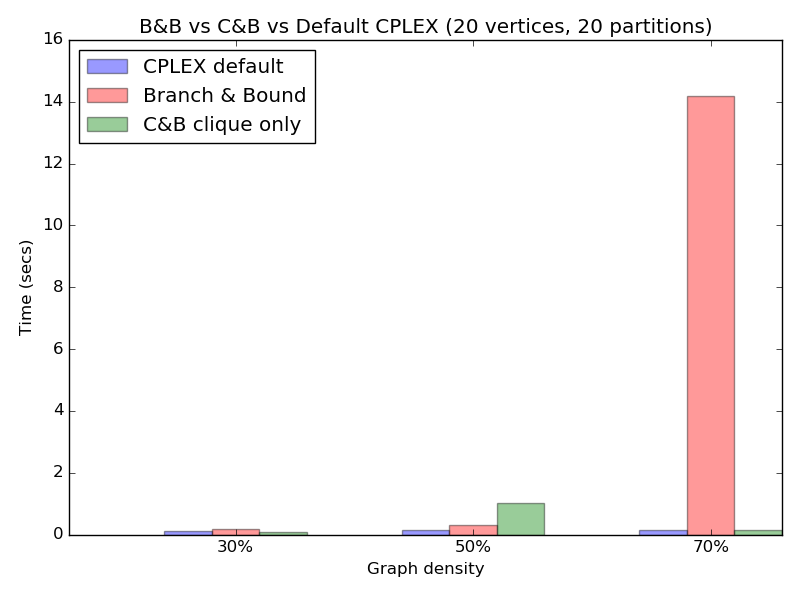
\includegraphics[width=\textwidth]{img/8-compare_v20_p20_i1_l40_t1_b0.png}
  \end{minipage}
  \begin{minipage}[b]{0.49\textwidth}
    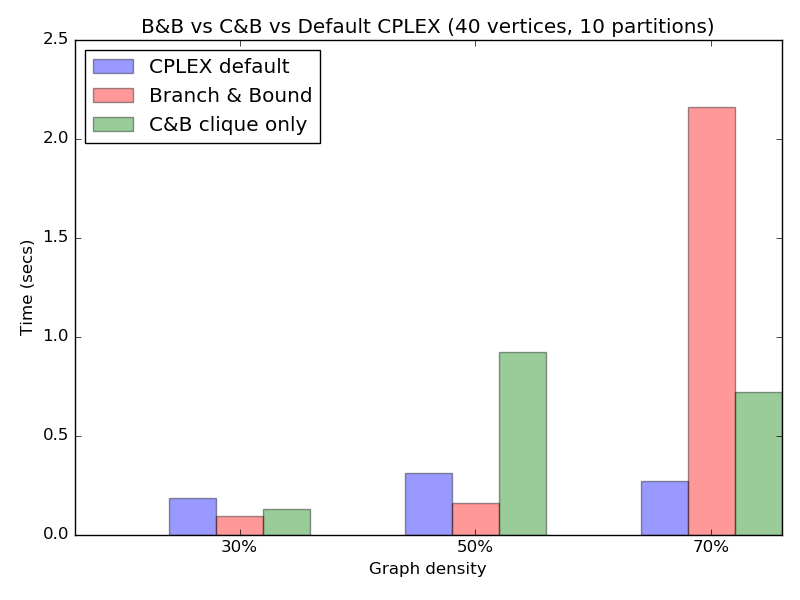
\includegraphics[width=\textwidth]{img/8-compare_v40_p10_i1_l40_t1_b0.png}
  \end{minipage}
  \hfill
  \begin{minipage}[b]{0.49\textwidth}
    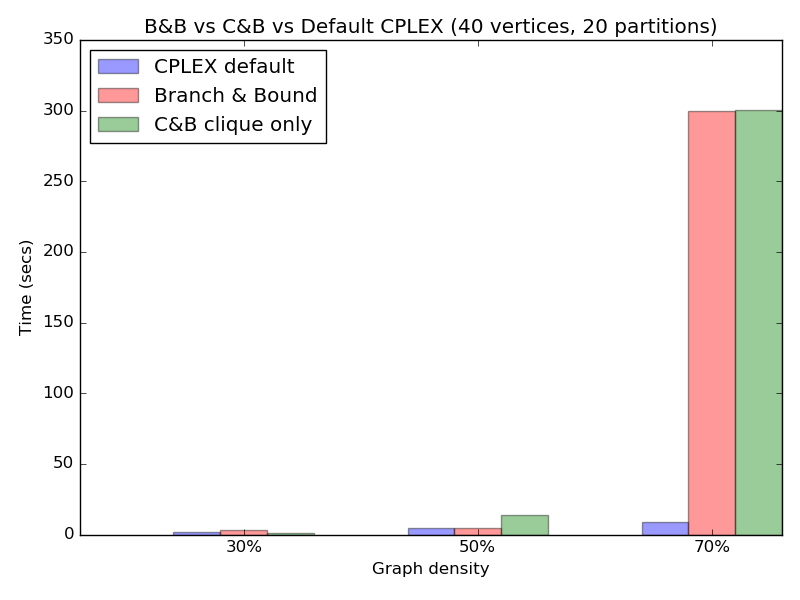
\includegraphics[width=\textwidth]{img/8-compare_v40_p20_i1_l40_t1_b0.png}
  \end{minipage}
	\caption{Comparacion B\&B, C\&B, CPLEX default para diferentes grafos.}
\end{figure}

Dado que el CPLEX por default utiliza cortes de Gomory y preprocesamiento de variables, no nos sorprende que en general sea superior a nuestras otras estrategias para grafos densos. Una propuesta interesante podría ser repetir esta experimentación permitiendo los cortes y el preprocesamiento para todas nuestras estrategias. Otra observación, el gráfico superior derecho es el caso de coloreo de grafos, dado que cada vértice pertenece a una partición diferente. Aquí podemos ver que las desigualdades de clique son sumamente útiles. 
